\documentclass{article}
\usepackage{amsmath}
\usepackage{breqn}
\usepackage{amssymb}

% FOR INSERTING IMAGES
\usepackage{graphicx}
\graphicspath{C:\Users\edgar\OneDrive\Documents\Code\OptRLResearch\IMC\manuals}

\title{A question in auction theory}
\author{Edgar Maddocks}
\date{April 2024}

\begin{document}
\maketitle

\section*{Introduction}
\begingroup
This short article will go through a challenging question taken from the first round of the manual section of
IMC's Prosperity 2 trading challenge. The question requires knowledge of probability 
distributions, some basic integration and also how to locate stationary points using 
partial differentiation. The main backstory to the Prosperity challenge is that you have been placed
on a tropical island with lots of different objects and materials, from which you must try to trade and make as
much profit as possible - in the currency of seashells. 

The question for this article says that lots of goldfish have 
arrived at the island with scuba gear that they would like to sell. But only at the right price. We do not know 
how many goldfish there are, however, we do know that there is constant demand for scuba gear on the island, 
at the price of \textbf{1000} seashells. You have the ability to make \textbf{two} offers to the fish, 
a lower offer, and a higher offer. Each fish will have a reserve price and for each fish you will first pose 
your lower offer. If this offer  is greater than there reserve price then a trade is made, and your profit is
\textbf{1000 - the price of your lower offer}. However, if your lower offer is not greater than the fishes reserve
price then you shall pose your higher offer, and again if this is greater than the reserve price, a trade is made
and your profit is \textbf{1000 - the price of your higher offer}. The two offer prices are the same for every fish.
\textit{Your goal is to set prices that ensure a profitable trade with as many goldfish as possible.}

The only information we are given is the distribution of the fishes' reserve prices.
\textbf{'The reserve price will be no lower than 900 and no higher than 1000. The 
probability scales linearly from least likely at 900 to most likely at 1000.'} And that 
\textbf{at the price of 900, the probability is 0}.
\\
\\
\textbf{Note:} the reserve prices are \textbf{real} values, while bid prices can only be
\textbf{integer} values.
\endgroup

\section*{Solution}
\indent Firstly, we will define the probability density function of the reserve prices to be 
$P(x)$, where $x$ is a reserve price in the interval $[900, 1000]$. We are told that $P(x)$
scales \textbf{linearly}, and therefore it is in the form: $ax + b$. So now let's write down
everything we know:
\setlength{\jot}{15pt} % set spacing between eqs. to 15pt
\begin{gather}
    P(x) = ax + b \\
    P(900) = 900a + b = 0 \\
    \int_{900}^{1000}P(x)dx = 1
\end{gather}

The last equation here is simply stating that the sum of all the probabilities of the reserve 
prices will be equal to one.

Solving this integral:
\begin{gather}
    \int_{900}^{1000}P(x)dx = 1 \\
    = \int_{900}^{1000}(ax+b)dx = 1 \\
    = \left[\frac{1}{2}ax^2 + bx\right]_{900}^{1000} = 1 \\
    = (500000a + 1000b) - (405000a + 900b) = 1 \\
    = 95000a + 100b = 1
\end{gather}

Now using equation $(8)$ and $(2)$ we can solve simultaneously to find the values of $a$ and $b$.

First multiplying equation $2$ by $100$
\begin{gather}
    90000a + 100b = 0
\end{gather}
Subtracting $(9)$ from $(8)$
\begin{gather}
    5000a = 1 \\
    \implies a = \frac{1}{5000}
\end{gather}
Now substituting back into $2$
\begin{gather}
    \frac{900}{5000} + b = 0 \\
    \implies b = -\frac{9}{50} 
\end{gather}

Now that we have the unique values of $a$ and $b$, we can redefine $P(x)$ in terms of these values.
\begin{gather}
    P(x) = \frac{1}{5000}x - \frac{9}{50}
\end{gather}

With the distribution now well-defined, we need a way to calculate our expected profit for any given
bids.
So we will define a profit function $Prof(b_1, b_2)$ where $b_1$ is our lower offer, and $b_2$ is our
higher offer. We will also let $Y$ be a random reserve price from the distribution.
\begin{equation}
    Prof(b_1, b_2) = 
    \left\{
        \begin{array}{lr}
            1000 - b_1, & Y < b_1 \\
            1000 - b_2, & b_1 < Y < b_2 \\
            0, & otherwise
        \end{array}
    \right\}
\end{equation}
Now, in place of taking a random sample $(Y)$ we can instead multiply the profit by the probability of $Y$ being less
than our offers.
Which will give us an expected value of the profit function
\begin{equation}
    \mathbb{E}[Prof(b_1, b_2)] = (1000 - b_1)(P(Y < b_1)) + (1000 - b_2)(P(b_1 < Y < b_2))
\end{equation}
Then, using $P(x)$ which we defined earlier, we can determine $P(Y < b_1)$
\begin{gather}
    P(Y < b_1) = \int_{900}^{b_1}P(x)dx \\
    = \int_{900}^{b_1}(\frac{1}{5000}x-\frac{9}{50})dx \\
    = \left[
        \frac{1}{10000}x^2 - \frac{9}{50}x
    \right]_{900}^{b_1} \\
    = \frac{1}{10000}b_1^2 - \frac{9}{50}b_1 + 81
\end{gather}
We can use the same method as above to also determine $P(b_1 < Y < b_2)$
\begin{gather}
    P(b_1 < Y < b_2)
    = \left[
        \frac{1}{10000}x^2 - \frac{9}{50}x
    \right]_{b_1}^{b_2} \\
    = \frac{1}{10000}b_2^2 - \frac{9}{50}b_2 - \frac{1}{10000}b_1^2
    + \frac{9}{50}b_1
\end{gather}
Now using these expressions, we can rewrite $\mathbb{E}[Prof(b_1, b_2)]$
\begin{dmath}
    \mathbb{E}[Prof(b_1, b_2)] = (1000 - b_1)\left(\frac{1}{10000}b_1^2 - \frac{9}{50}b_1 + 81\right)
    + (1000 - b_2)\left(\frac{1}{10000}b_2^2 - \frac{9}{50}b_2 - \frac{1}{10000}b_1^2 + \frac{9}{50}b_1\right)
\end{dmath}
$\mathbb{E}[Prof(b_1, b_2)]$ is now our objective function to maximize, and I will refer to it as $O(b_1, b_2)$
for ease of notation.

Our goal was to maximize profits from our trading. We can therefore reframe this as maximizing our
objective function with respect to $b_1$ and $b_2$. Firstly, we can actually plot this function as a surface,
with $x$ and $y$ as our two bids, and $z$ as the value of our objective function (expected profit) with these
bid values and this will give us a good visualization of our problem.

\begin{figure}[h!]
    \centering
    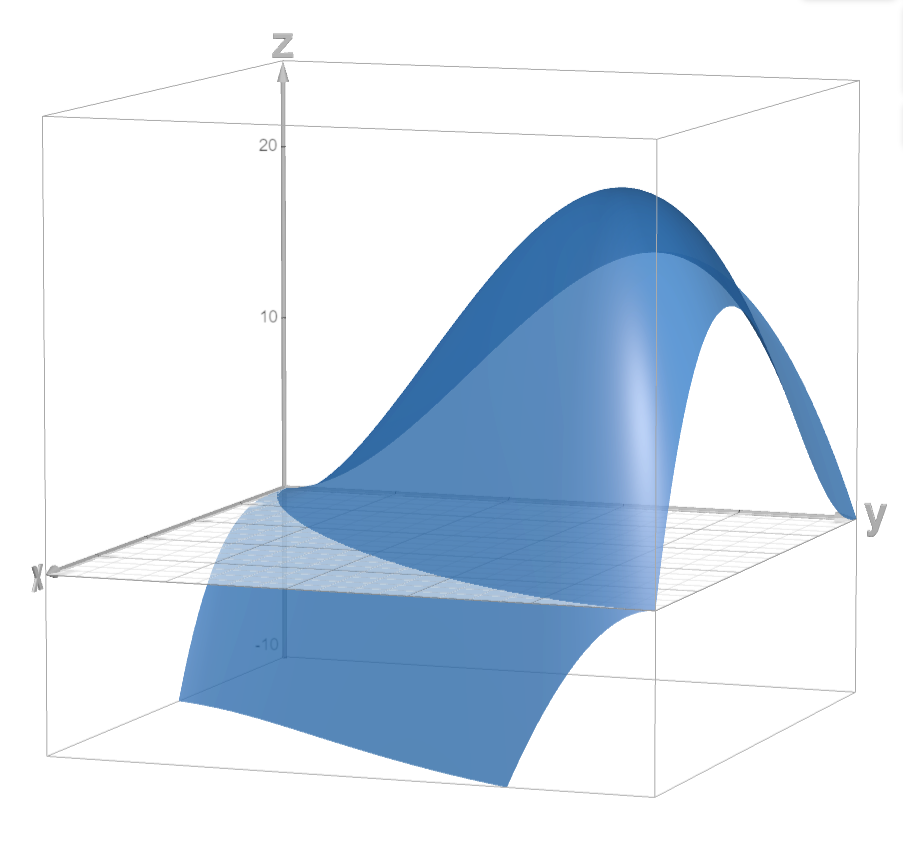
\includegraphics[scale = 0.4]{O(b_1, b_2) plot.png}
    \caption{Plot of objective function with $b_1$ and $b_2$ values in the range $[900,1000]$ in Desmos}
\end{figure}

Now, with this visualization, we can clearly see the shape of the objective function and the maxima that we are
trying to locate. To determine the location of a stationary point on a surface, we can take the partial derivatives
of $O(b_1, b_2)$ with respect to each input $(b_1, b_2)$ and set both equal to zero.
\begin{gather}
    \frac{\partial O}{\partial b_1} = - \frac{3}{10000}b_1^2 + \frac{2}{10000}b_1b_2 + \frac{9}{25}b_1 - \frac{9}{50}b_2 - 81 \\
    \frac{\partial O}{\partial b_2} = \frac{1}{10000}b_1^2 - \frac{3}{10000}b_2^2 - \frac{9}{50}b_1 + \frac{14}{25}b_2 - 180
\end{gather}
Setting both expressions equal to zero and solving simultaneously
\begin{gather}
    \frac{\partial O}{\partial b_1} = 0 \\
    \frac{\partial O}{\partial b_2} = 0
\end{gather}
Rearranging $(24)$ for $b_2$
\begin{gather}
    \frac{2}{10000}b_1b_2 - \frac{9}{50}b_2 = \frac{3}{10000}b_1^2 - \frac{9}{25}b_1 + 81 \\
    2b_1b_2 - 1800b_2 = 3b_1^2 - 3600b_1 + 8100000 \\
    b_2 = \frac{3b_1^2 - 3600b_1 + 8100000}{2(b_1 - 900)}, b_1 \neq 900 \\
    b_2 = \frac{3(b_1^2 - 1200b_1 + 2700000)}{2(b_1 - 900)}, b_1 \neq 900 \\
    b_2 = \frac{3((b_1 - 300)(b_1 - 900))}{2(b_1 - 900)}, b_1 \neq 900 \\
    b_2 = \frac{3(b_1 - 300)}{2}, b_1 \neq 900
\end{gather}
Substituting back into $(25)$
\begin{dmath}
    \frac{1}{10000}b_1^2 - \frac{3}{10000}\left(\frac{3(b_1 - 300)}{2}\right)^2 - \frac{9}{50}b_1 + \frac{14}{25}\left(\frac{3(b_1 - 300)}{2}\right) - 180 = 0
\end{dmath}
Simplifying and solving for $b_1$
\begin{gather}
    b_1^2 - \frac{27(b_1-300)^2}{4} - 1800x + 8400(b_1-300) - 1800000 = 0 \\
    -\frac{23b_1^2}{4} + 10650b_1 - 4927500 = 0 \\
    b_1 = \frac{-10650\pm 300}{2(-\frac{23}{4})} \\
    b_1 = 900 \: \text{ or } \: b_1 = \frac{21900}{23}
\end{gather}
When we defined $b_2$ in terms of $b_1$ in equation $(33)$, we acknowledged that
$b_1$ cannot equal $900$. Therefore, our only solution for $b_1$ is $\frac{21900}{23} \approx 952.17$.
Substituting this back into $(24)$
\begin{gather}
    -\frac{3}{10000}\left(\frac{21900}{23}\right)^2 + \frac{2}{10000}\frac{21900}{23}b_2+\frac{9}{25}\frac{21900}{23} - \frac{9}{50}b_2 - 81 = 0
\end{gather}
Simplifying and solving for $b_2$
\begin{gather}
    -\frac{143883}{529} + \frac{219}{1150}b_2 + \frac{7884}{23} - \frac{9}{50}b_2 - 81 = 0\\
    \frac{6}{575}b_2 - \frac{5400}{529} = 0 \\
    \implies b_2 = \frac{22500}{23} \\
    b_2 \approx 978.26
\end{gather}

\section*{Checks}
Now we have solved for our two offers which maximize our objective function.
However, if you remember, our bids must be integers. Therefore, we could just round
to the nearest integer, giving values of $b_1 = 952$ and $b_2 = 978$, however I will
complete a small grid search to ensure the rounding produces the optimal values.

The lower value for $b_1$ will be $952$, and the upper value will be $953$. As for $b_2$,
the lower value will be $978$, and the upper value $979$.

Creating our grid
\begin{center}
    \begin{tabular}{ |c|c|c| }
        \hline
        $O(b_1, b_2)$& 952 & 953 \\
        \hline
        978 & & \\
        \hline
        979 & & \\
        \hline
    \end{tabular}
\end{center}

Now for each pair in the grid, we can substitute the values into our 
objective function as $b_1$ and $b_2$. Doing so produces the following results
\begin{center}
    \begin{tabular}{ |c|c|c| }
        \hline
        $O(b_1, b_2)$ & 952 & 953 \\
        \hline
        978 & 20.4152 & 20.4073 \\
        \hline
        979 & 20.4069 & 20.4095 \\
        \hline
    \end{tabular}
\end{center}

After completing this quick grid search, we get the final result that the optimal value for
$b_1$ is $952$, and the optimal value for $b_2$ is $978$.

\section*{Simulation}
After creating a simulation to run locally in the form of a basic python script, I 
completed an exhaustive grid search, as well as a SciPy optimization. 

I first chose to run the simulation on 1 million samples from the distribution, and then 
generated random reserve prices by first generating random values in the range $[0, 1]$ and 
then using the inverse of the cumulative distribution function of reserve prices to 
generate the reserve price samples. 

For the grid search, I then created a list of tuples which contained every combination 
of different low and high offers. This resulted in just over 5000 different combinations 
of prices. After evaluating each of these pairs on 1 million samples, the best performing 
pair was also $(952, 978)$. With a simulated profit per fish of 20.4195. This search took 
approx. 60.2 seconds.

\textbf{Note:} After rerunning this search with 10 samples, pair $(952, 978)$ was still the 
highest performing, scoring a profit per fish of 20.4218. With the simulation taking 828 seconds 
(13 minutes 48 seconds).
\\
\\
\indent Now, using the minimize function from SciPy.optimize, with the metric being to minimize 
the negative profit per fish i.e. maximize profit per fish on 1 million samples, the optimal pair 
is yet again (952.2, 978.2). With a profit per fish of 20.3968.

\textbf{Note:} After running this simulation again with 10 million samples, the optimal pair was again 
$(952.2 ,978.2)$

\section*{Conclusion}
A lower bid of 952 and a higher bid of 978 is most certainly the optimal answer for this question, 
averaging a profit per fish of ~20.4 on large sample sizes of reserve prices. Backed up by not only 
closed-form solutions, but also exhaustive grid-search and computational optimization.













\end{document}